% !TeX root = ../alda_g17.tex

\tableofcontents

\chapter{Introduction}

\section{Descripción del problema}
La captura de movimiento markerless (sin marcadores físicos) representa una línea activa de investigación en visión artificial con aplicaciones en robótica, rehabilitación médica, interfaces humano-máquina e interacción natural. \cite{Pauzietal2021}

Los enfoques tradicionales basados en sensores físicos, trajes de captura óptica o cámaras de profundidad resultan costosos e intrusivos. El presente proyecto propone un sistema basado exclusivamente en una cámara convencional que, procesando el video en tiempo real, detecte la pose del brazo humano, calcule los ángulos articulares de hombro, codo y muñeca, y transfiera esos valores a la simulación visual de un brazo robótico virtual de tres grados de libertad (GDL).  \cite{Vintimilla2026}

La solución adopta MediaPipe Pose de Google, un framework de código abierto que proporciona detección de 33 landmarks corporales en tiempo real sin necesidad de GPU, combinado con OpenCV para la adquisición y el procesamiento de imagen. \cite{Bazarevskyetal2020} \cite{Lugaresietal2019}

\subsection*{Diagrama de Bloques General del Sistema}
La figura \ref{fig:diagrama_bloques} representa el flujo de datos global del proyecto, descompuesto en sus cinco módulos funcionales principales.

\begin{figure}[h!]
    \centering
    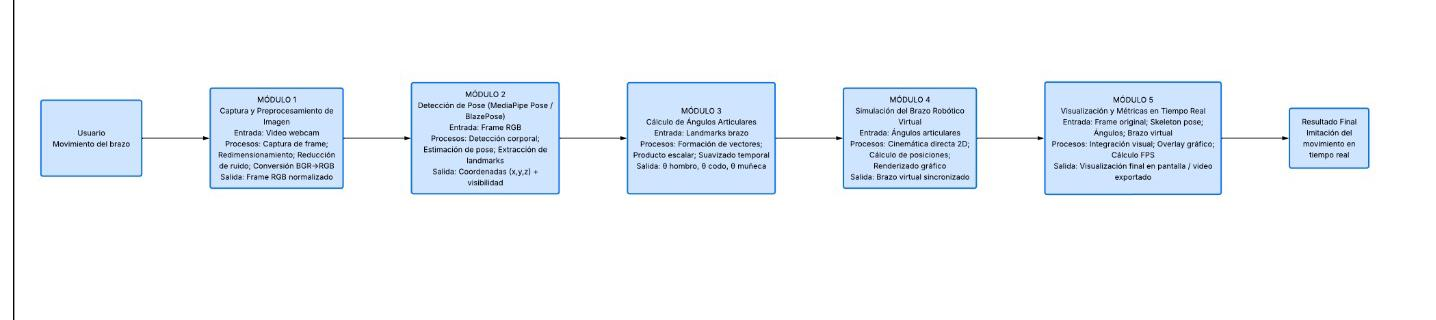
\includegraphics[width=1\textwidth]{images/diagrama_bloques.jpeg}
    \caption{Diagrama de bloques del sistema de imitación de movimientos con MediaPipe Pose.}
    \label{fig:diagrama_bloques}
\end{figure}

Cada bloque representa un módulo funcional independiente con entradas y salidas definidas. El video de la cámara entra al sistema por M1, los landmarks son extraídos en M2, los ángulos se calculan en M3, el brazo robótico es simulado en M4 y todo se integra visualmente en M5. \cite{Bazarevskyetal2020} \cite{Bradski2000}
\section{Justificación del problema}
MediaPipe fue presentado originalmente como un framework modular para construir pipelines de percepción reproducibles entre plataformas. Su componente BlazePose amplió esta capacidad al dominio de la estimación de pose corporal en tiempo real, logrando latencias menores a 30 ms en CPU mediante un pipeline de dos etapas: detector de persona (BlazePose Detector) y estimador de pose (BlazePose Estimator) que extrae 33 puntos clave. \cite{Bazarevskyetal2020} \cite{Lugaresietal2019}

Trabajos previos como los de Pauzi et al. (2021) demostraron la efectividad de BlazePose para estimar movimientos corporales con una diferencia de precisión dentro del 10\% respecto a sistemas IMU de referencia. En el dominio de la teleoperación robótica, Altayeb (2023) implementó un sistema de replicación de gestos de mano en un brazo robótico usando MediaPipe Hands, validando la viabilidad de este enfoque para control de actuadores virtuales. \cite{Pauzietal2021} \cite{Altayeb2023}

La justificación económica radica en el bajo costo de implementación: el sistema requiere únicamente una webcam USB estándar ($<$ \$20 USD), sin sensores de profundidad ni hardware especializado. El stack de software es completamente open-source (Python, OpenCV, MediaPipe, NumPy).

\section{Objetivos}

\subsection{Objetivo principal}
Desarrollar un sistema de visión artificial que, a partir de video capturado en tiempo real por una cámara convencional, detecte los movimientos del brazo humano utilizando MediaPipe Pose \cite{Bazarevskyetal2020} \cite{Lugaresietal2019}, calcule los ángulos de las articulaciones hombro, codo y muñeca, y los transfiera a la simulación visual sincronizada de un brazo robótico virtual de 3 GDL.

\subsection{Objetivos específicos}
\begin{enumerate}
    \item Implementar un módulo de captura y preprocesamiento de video en tiempo real usando OpenCV \cite{Bradski2000} con soporte para normalización de resolución (640×480) y conversión de espacio de color BGR→RGB.
    \item Integrar el modelo MediaPipe Pose \cite{Bazarevskyetal2020} para la detección y extracción de los 33 landmarks corporales, con énfasis en los puntos clave del brazo (hombros: landmarks 11,12; codos: 13,14; muñecas: 15,16).
    \item Desarrollar un módulo de cálculo de ángulos articulares mediante álgebra vectorial (producto escalar y norma de vectores) para los tres GDL del brazo: hombro (elevación), codo (flexión) y muñeca (flexión), con filtrado de media móvil de 5 frames.
    \item Implementar la simulación 2D del brazo robótico virtual mediante cinemática directa, renderizando en tiempo real el modelo sobre el frame de video usando primitivas OpenCV (cv2.line, cv2.circle) \cite{Bradski2000}.
    \item Construir un módulo de visualización integrada que muestre el skeleton de MediaPipe \cite{Lugaresietal2019}, los ángulos articulares calculados, el brazo robótico simulado y métricas de rendimiento (FPS).
    \item Evaluar el desempeño del sistema con métricas de latencia (FPS objetivo: $\geq$ 20 FPS), precisión angular y estabilidad del sistema ante variaciones de iluminación, usando como referencia el benchmark del dataset COCO Keypoints \cite{10.1007/978-3-319-10602-1_48}.
\end{enumerate}

\section{Módulos del proyecto}
El sistema se descompone en cinco módulos funcionales interconectados. La arquitectura modular facilita el desarrollo y prueba independiente de cada componente en el marco SCRUM adoptado. Las tecnologías principales son OpenCV \cite{Bradski2000} para procesamiento de imagen y MediaPipe Pose \cite{Bazarevskyetal2020, 10.1007/978-3-319-10602-1_48} para estimación de pose.

\subsection{Módulo 1 -- Captura y Preprocesamiento de Imagen}

\subsubsection*{Objetivo}
Adquirir el flujo de video en tiempo real desde la cámara y preparar
cada frame para su procesamiento posterior mediante normalización de
resolución, conversión de espacio de color y reducción de ruido.

\paragraph{Entradas y Salidas}

\begin{table}[h!]
\centering
\label{tab:m1_io}
\renewcommand{\arraystretch}{1.3}
\begin{tabularx}{\textwidth}{
    >{\bfseries}p{3cm}
    X
    X
}    
\toprule
&
\textbf{Descripción} &
\textbf{Formato / Especificación} \\
\midrule
Entrada &
  Flujo de video desde webcam USB o cámara integrada &
  Resolución variable (640$\times$480 -- 1920$\times$1080), 30~FPS \\
\midrule
Salida &
  Frame de imagen normalizado en espacio RGB &
  NumPy array RGB, resolución fija 640$\times$480, píxeles en $[0,\,255]$ \\
\bottomrule
\end{tabularx}
\caption{Entradas y salidas del Módulo 1.}
\end{table}

\paragraph{Herramientas Tecnológicas}
\begin{itemize}[leftmargin=1.5em]
  \item \textbf{Software:} Python~3.10+ como lenguaje de implementación.
  \item \textbf{Librería principal:} OpenCV (cv2~v4.8+) \cite{Bradski2000}
        — captura de video (cv2.VideoCapture), redimensionado
        (cv2.resize) y conversión de espacio de color
        (cv2.cvtColor).
  \item \textbf{Librería de soporte:} NumPy (v1.24+) para manejo
        y operaciones sobre arrays de imagen.
\end{itemize}

\paragraph{Técnicas de Visión Computacional}
\begin{itemize}[leftmargin=1.5em]
  \item \textbf{Realzado y restauración:} aplicación opcional de filtro
        gaussiano (cv2.GaussianBlur) para atenuación de ruido
        de alta frecuencia antes de la inferencia de
        MediaPipe~\cite{GonzalezWoods2018}.
  \item Redimensionado con interpolación bicúbica
        (cv2.INTER\_CUBIC) para preservar calidad de bordes
        al escalar el frame.
  \item Conversión de espacio de color BGR$\to$RGB requerida por el
        modelo BlazePose de MediaPipe.
\end{itemize}

\subsection{Módulo 2 -- Detección de Pose con MediaPipe}
\subsubsection*{Objetivo}

Detectar los 33~landmarks del cuerpo humano en cada frame de video
utilizando el modelo MediaPipe~Pose (BlazePose), con énfasis en los
puntos clave del brazo: hombros (landmarks~11,~12), codos
(13,~14) y muñecas (15,~16)~\cite{Bazarevskyetal2020}.

\subsubsection*{Entradas y Salidas}

\begin{table}[h!]
\centering
\label{tab:m1_io}
\renewcommand{\arraystretch}{1.3}
\begin{tabularx}{\textwidth}{
    >{\bfseries}p{3cm}
    X
    X
}    
\toprule
&
\textbf{Descripción} &
\textbf{Formato / Especificación} \\
\midrule
Entrada &
  Frame RGB preprocesado (salida de M1) &
  NumPy array RGB 640$\times$480 \\
\midrule
Salida &
  33~landmarks corporales con visibilidad &
  \texttt{NormalizedLandmarkList}: coord.\
  $(x,\,y,\,z) \in [0,1]$ + visibilidad $\in [0,1]$
  por punto \\
\bottomrule
\end{tabularx}
\caption{Entradas y salidas del Módulo 2.}
\end{table}
 
\paragraph{Herramientas Tecnológicas}
\begin{itemize}[leftmargin=1.5em]
  \item \textbf{Modelo de IA preentrenado:}
        MediaPipe~Pose (BlazePose)~v0.10+~\cite{Bazarevskyetal2020,Lugaresietal2019}
        — modelo de estimación de pose de 33~landmarks entrenado sobre
        el dataset COCO~Keypoints. No requiere GPU.
  \item \textbf{Framework:} MediaPipe (Google) \cite{Lugaresietal2019}
        — framework de construcción de pipelines de percepción con
        soporte cross-platform.
  \item \textbf{Librería de soporte:} NumPy para extracción y
        transformación de las coordenadas de landmarks al espacio de
        píxeles.
\end{itemize}
 
\paragraph{Técnicas de Visión Computacional}
\begin{itemize}[leftmargin=1.5em]
  \item \textbf{Pipeline BlazePose de dos etapas:}
        \begin{enumerate}[leftmargin=2em]
          \item Detector de persona que delimita el bounding
                box de la región de interés.
          \item Estimador de pose que infiere los 33 landmarks con
                alta precisión dentro de esa región.
        \end{enumerate}
  \item \textbf{Modo de video} (static\_image\_mode=False):
        el modelo aprovecha la coherencia temporal entre frames
        consecutivos para acelerar la inferencia y estabilizar los
        landmarks.
  \item \textbf{Extracción de landmarks de interés:} se seleccionan los
        índices 11–16 (hombros, codos, muñecas) de los 33~puntos
        detectados para alimentar el módulo de cálculo angular.
\end{itemize}

\subsection{Módulo 3 -- Cálculo de Ángulos Articulares}
\subsubsection*{Objetivo}
Calcular los ángulos de flexión/extensión en las articulaciones
hombro, codo y muñeca a partir de las coordenadas 2D de los landmarks,
usando la definición vectorial del ángulo entre dos segmentos
articulares.

\subsubsection*{Entradas y Salidas}

\begin{table}[h!]
\centering
\label{tab:m1_io}
\renewcommand{\arraystretch}{1.3}
\begin{tabularx}{\textwidth}{
    >{\bfseries}p{3cm}
    X
    X
}    
\toprule
&
\textbf{Descripción} &
\textbf{Formato / Especificación} \\
\midrule
Entrada &
  Coordenadas 2D de hombro, codo y muñeca (salida de M2) &
  Pares $(x,\,y)$ en píxeles para cada articulación
  (landmarks 11–16) \\
\midrule
Salida &
  Tripleta de ángulos articulares suavizados &
  $\theta_{\text{hombro}},\,\theta_{\text{codo}},\,
   \theta_{\text{muñeca}}$ en grados $[0°,\,180°]$ (float64) \\
\bottomrule
\end{tabularx}
\caption{Entradas y salidas del Módulo 3.}
\end{table}

\paragraph{Herramientas Tecnológicas}\mbox{}

\begin{itemize}[leftmargin=1.5em]
  \item \textbf{Librería principal:} NumPy (v1.24+) para
        cálculo del producto escalar (np.dot), norma de
        vectores (np.linalg.norm) y función
        arccos (np.arccos) necesarios en la fórmula
        angular.
  \item \textbf{Librería de soporte:} Matplotlib (v3.7+)
        para graficar la evolución temporal de los ángulos articulares
        durante las pruebas y análisis de resultados.
\end{itemize}
 
\paragraph{Técnicas de Visión Computacional y Geometría}
\begin{itemize}[leftmargin=1.5em]
  \item \textbf{Cálculo de ángulos mediante producto escalar:}
        \cite{GonzalezWoods2018}
 
        \begin{equation}
            \theta \;=\; \arccos{ \frac{\vec{v}_1 \cdot \vec{v}_2}{|\vec{v}_1|\,|\vec{v}_2|} }
            \label{eq:angulo}
        \end{equation}

        donde $\vec{v}_1$ y $\vec{v}_2$ son los vectores que forman
        cada par de segmentos en la articulación.

  \item \textbf{Filtrado temporal con media móvil} de ventana $w = 5$
        frames para suavizar fluctuaciones por ruido de detección de
        BlazePose y evitar movimientos bruscos en la simulación del
        brazo robótico.
  \item \textbf{Cálculo de vectores entre articulaciones:} diferencia
        de coordenadas entre el landmark proximal y el distal para
        construir cada vector de segmento corporal.
\end{itemize}
 

\subsection{Módulo 4 -- Simulación del Brazo Robótico Virtual}

\subsubsection*{Objetivo}
Representar y animar en pantalla un brazo robótico de 3~GDL cuyas
posiciones articulares se corresponden directamente con los ángulos
calculados por M3, logrando una imitación visual sincronizada en
tiempo real~\cite{Altayeb2023}.

\subsubsection*{Entradas y Salidas}

\begin{table}[h!]
\centering
\label{tab:m1_io}
\renewcommand{\arraystretch}{1.3}
\begin{tabularx}{\textwidth}{
    >{\bfseries}p{3cm}
    X
    X
}    
\toprule
&
\textbf{Descripción} &
\textbf{Formato / Especificación} \\
\midrule
Entrada &
  Ángulos articulares suavizados (salida de M3) &
  $\theta_{\text{hombro}},\,\theta_{\text{codo}},\,
   \theta_{\text{muñeca}}$ en grados (float64) \\
\midrule
Salida &
  Frame con overlay del brazo robótico virtual &
  NumPy array BGR con eslabones y articulaciones renderizados
  en tiempo real \\
\bottomrule
\end{tabularx}
\caption{Entradas y salidas del Módulo 4.}
\end{table}
 
\paragraph{Herramientas Tecnológicas}
\begin{itemize}[leftmargin=1.5em]
  \item \textbf{Librería principal:}
        OpenCV (cv2)~\cite{Bradski2000} para renderizado
        de primitivas gráficas: cv2.line (eslabones),
        cv2.circle (articulaciones),
        cv2.putText (ángulos).
  \item \textbf{Librería de soporte:} NumPy para el cálculo
        de coordenadas cartesianas de cada articulación mediante
        cinemática directa 2D.
\end{itemize}

\paragraph{Técnicas de Visión Computacional y Robótica}
\begin{itemize}[leftmargin=1.5em]
  \item \textbf{Cinemática directa 2D:} a partir de los ángulos
        articulares y las longitudes de eslabón predefinidas
        ($L_{\text{hombro}}$, $L_{\text{antebrazo}}$,
        $L_{\text{mano}}$), se calculan las posiciones cartesianas
        $(x,\,y)$ de cada junta del brazo virtual mediante relaciones
        trigonométricas acumulativas:
 
        \begin{align}
          x_1 &= x_0 + L_{\text{hombro}}\cos(\theta_{\text{hombro}})
          \notag \\
          y_1 &= y_0 - L_{\text{hombro}}\sin(\theta_{\text{hombro}})
          \notag \\
          x_2 &= x_1 + L_{\text{antebrazo}}
                        \cos(\theta_{\text{hombro}}
                             + \theta_{\text{codo}})
          \notag \\
          y_2 &= y_1 - L_{\text{antebrazo}}
                        \sin(\theta_{\text{hombro}}
                             + \theta_{\text{codo}})
          \label{eq:cinematica}
        \end{align}
 
  \item \textbf{Renderizado de overlay:} el brazo robótico se
        dibuja sobre el frame de video como una capa superpuesta,
        permitiendo la comparación visual directa entre el movimiento
        humano y la imitación del brazo virtual.
\end{itemize}

\subsection{Módulo 5 -- Visualización y Métricas en Tiempo Real}

\subsubsection*{Objetivo}
Integrar y mostrar en una ventana unificada el frame original anotado
con el skeleton de MediaPipe, los ángulos calculados, el
brazo robótico virtual y las métricas de rendimiento del sistema
(FPS).

\subsubsection*{Entradas y Salidas}

\begin{table}[h!]
\centering
\label{tab:m1_io}
\renewcommand{\arraystretch}{1.3}
\begin{tabularx}{\textwidth}{
    >{\bfseries}p{3cm}
    X
    X
}    
\toprule
&
\textbf{Descripción} &
\textbf{Formato / Especificación} \\
\midrule
Entrada &
  Frame original $+$ landmarks $+$ ángulos $+$
  overlay del brazo robótico &
  Salidas de M1, M2, M3 y M4 en cada iteración del
  bucle principal \\
\midrule
Salida &
  Frame anotado final visualizado en tiempo real &
  Ventana OpenCV (cv2.imshow) con overlay
  completo; exportación opcional a MP4
  (cv2.VideoWriter) \\
\bottomrule
\end{tabularx}
\caption{Entradas y salidas del Módulo 5.}
\end{table}
 
\paragraph{Herramientas Tecnológicas}
\begin{itemize}[leftmargin=1.5em]
  \item \textbf{Librería principal:}
        OpenCV (cv2)~\cite{Bradski2000} — visualización
        en ventana interactiva (cv2.imshow,
        cv2.waitKey) y exportación de video
        (cv2.VideoWriter).
  \item \textbf{MediaPipe Drawing Utils}~\cite{Lugaresietal2019}
        — dibujo automático del skeleton de 33~landmarks y
        conexiones corporales sobre el frame.
  \item Matplotlib (v3.7+) — generación de gráficas de
        evolución temporal de ángulos articulares y métricas de FPS
        para análisis de resultados.
  \item scikit-learn (v1.3+) — cálculo de métricas
        estadísticas de evaluación: error medio angular (MAE),
        correlación de Pearson y análisis de estabilidad del sistema.
\end{itemize}
 
\paragraph{Técnicas de Visión Computacional}
\begin{itemize}[leftmargin=1.5em]
  \item \textbf{Cálculo de FPS en tiempo real:} medición del tiempo
        de procesamiento por frame con timestamps de Python
        (time.time()) para monitoreo continuo del rendimiento
        del sistema.
  \item \textbf{Visualización compuesta:} superposición de múltiples
        capas (frame original, skeleton MediaPipe,
        overlay robótico, texto de métricas) mediante
        operaciones de blendingde OpenCV.
\end{itemize}

\section{Soluciones existentes}

Hoy en día, replicar los movimientos del cuerpo humano mediante visión por computadora es un campo clave para disciplinas como la robótica, la interacción persona-ordenador, la medicina de rehabilitación y la automatización. En la literatura actual encontramos diferentes estrategias para resolver esto, pero casi todas comparten el mismo fin: capturar lo que hace un usuario, calcular dónde están sus articulaciones en el espacio y trasladar esa información a un robot o a un entorno digital.

Una de las líneas de investigación con más fuerza es la teleoperación por imitación. Aquí el reto principal no es solo registrar el movimiento de los brazos o piernas del usuario, sino ver cómo adaptar esos datos a la estructura de un robot, cuyas articulaciones y límites físicos suelen ser muy diferentes a los de un humano.

Por ejemplo, Zhang y su equipo diseñaron un sistema para conectar los movimientos de un brazo humano con un robot industrial. Lo interesante de su propuesta es que crearon un modelo cinemático capaz de traducir las trayectorias en tiempo real; el robot lograba replicar la orientación del brazo incluso teniendo una anatomía completamente distinta \cite{Wang2020Fast}. Esto demostró que la compatibilidad física no es una barrera insalvable. En una línea parecida, Xuan y Tang apostaron por la simplicidad del hardware al usar una sola cámara web común (óptica monocular) para controlar un brazo robótico \cite{xuan2017vision}. Su trabajo dejó claro que no hacen falta sensores pegados al cuerpo ni trajes especiales si se cuenta con un buen procesamiento visual.

Por otro lado, cuando se trabaja con robots humanoides, la complejidad aumenta. En otro estudio, Han et al. se enfocaron en este problema desarrollando un método para rastrear específicamente el codo y la muñeca del operario. Su sistema ajusta esas coordenadas sobre la marcha para que el robot aprenda tareas de manipulación sin perder el equilibrio ni la fluidez \cite{han2024robust}. Más recientemente, un estudio de la Universidad de los Andes (2026) propuso usar cámaras RGB-D (que miden profundidad) junto con algoritmos de estimación de pose. Su investigación confirmó que la visión artificial actual es lo suficientemente madura como para interactuar con gemelos virtuales y robots físicos con una precisión bastante aceptable, dejando atrás los incómodos sensores portables \cite{alibeigi2017inverse}.

Al revisar todas estas soluciones, salta a la vista que casi todos los autores siguen una misma receta: capturan el video, detectan los puntos clave del cuerpo, analizan la geometría del movimiento y lo envían al dispositivo. Sin embargo, hay un problema: casi toda la investigación actual se empeña en usar robots físicos caros o equipos muy específicos. Es justo ahí donde este proyecto quiere marcar la diferencia. En lugar de lidiar con hardware costoso, proponemos crear una simulación con un brazo robótico virtual. De esta forma, reducimos los costos y la complejidad técnica a cero, pero manteniendo el foco en lo importante: experimentar y validar algoritmos de visión artificial y procesamiento de imágenes en tiempo real.
